\documentclass[tikz,border=12pt]{standalone}
\usepackage{tikz}
\usetikzlibrary{shapes.geometric,arrows.meta,positioning,fit,backgrounds,calc}

\renewcommand{\familydefault}{\sfdefault}
\definecolor{cborder}{HTML}{1E293B}
\definecolor{cbg}{HTML}{F8FAFC}
\definecolor{cbox}{HTML}{FFFFFF}
\definecolor{cblue}{HTML}{1E40AF}
\definecolor{cbluelight}{HTML}{EFF6FF}
\definecolor{cgray}{HTML}{64748B}
\definecolor{caccent}{HTML}{0284C7}

\begin{document}
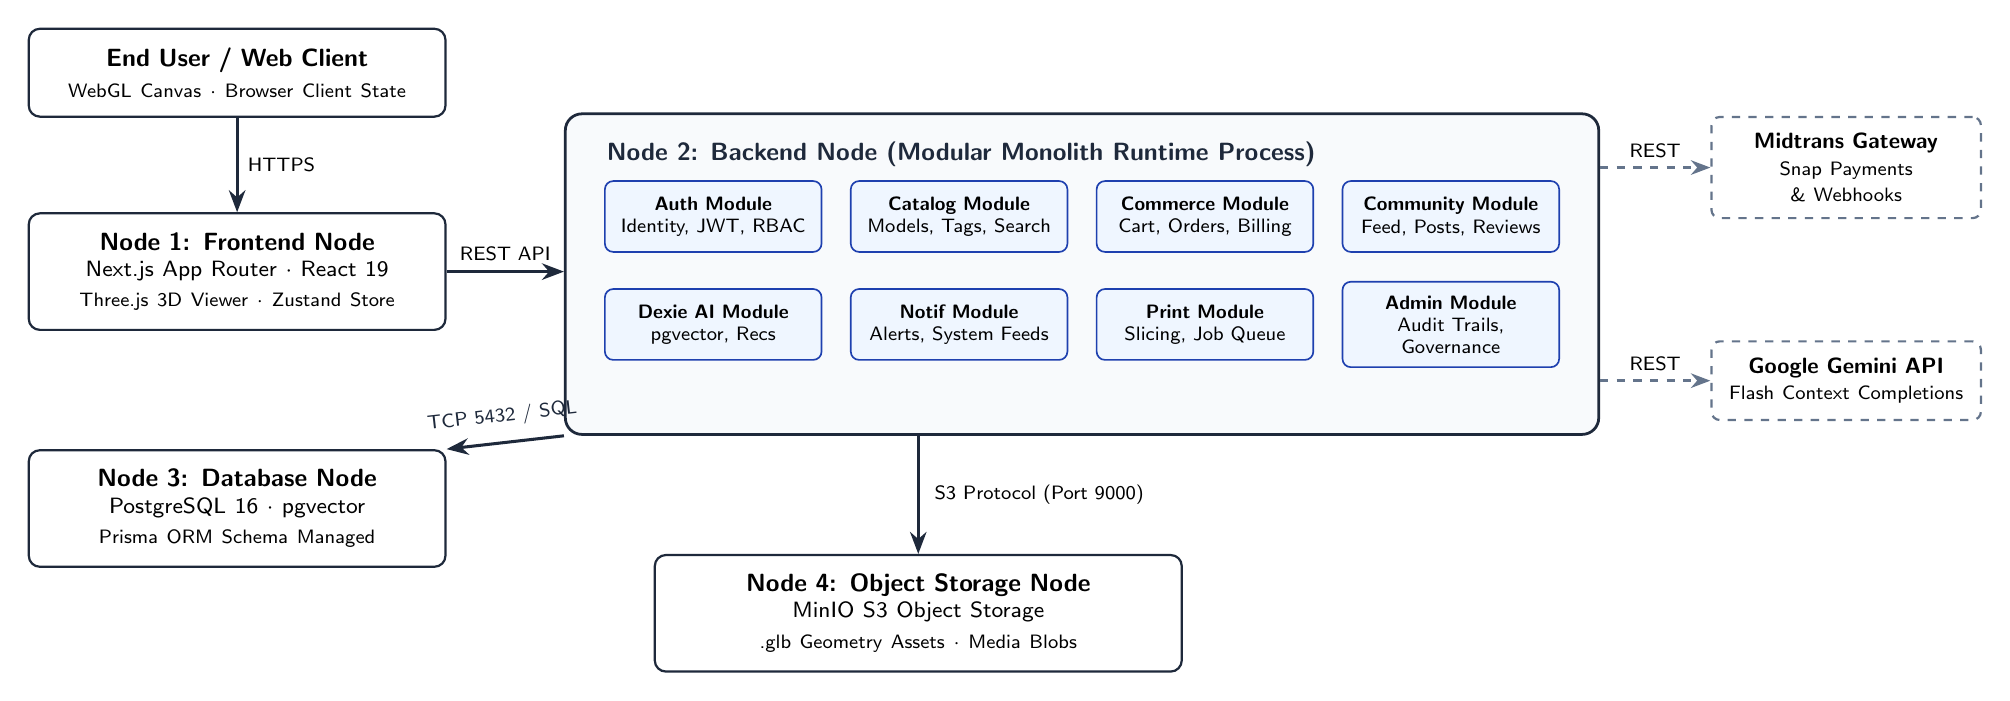
\begin{tikzpicture}[
    font=\small,
    >=Stealth,
    node distance=0.8cm and 1.0cm,
    comp/.style={
        draw=cborder,
        fill=cbox,
        rounded corners=4pt,
        line width=0.8pt,
        align=center,
        inner sep=7pt
    },
    mod/.style={
        draw=cblue,
        fill=cbluelight,
        rounded corners=3pt,
        line width=0.6pt,
        align=center,
        inner sep=5pt,
        font=\scriptsize,
        text width=2.4cm,
        minimum height=0.9cm
    },
    ext/.style={
        draw=cgray,
        fill=white,
        dashed,
        rounded corners=3pt,
        line width=0.8pt,
        align=center,
        inner sep=6pt,
        font=\footnotesize,
        text width=3.0cm
    },
    flow/.style={
        ->,
        line width=1.1pt,
        draw=cborder
    },
    dashedflow/.style={
        ->,
        line width=0.9pt,
        draw=cgray,
        dashed
    }
]

    % Client
    \node[comp, text width=4.8cm] (client) {
        \textbf{End User / Web Client}\\
        \scriptsize WebGL Canvas $\cdot$ Browser Client State
    };

    % Frontend Node
    \node[comp, below=1.2cm of client, text width=4.8cm] (frontend) {
        \textbf{Node 1: Frontend Node}\\
        \footnotesize Next.js App Router $\cdot$ React 19\\
        \scriptsize Three.js 3D Viewer $\cdot$ Zustand Store
    };

    % Backend Modules
    \node[mod, right=2.0cm of frontend, yshift=0.7cm] (m_auth) {\textbf{Auth Module}\\Identity, JWT, RBAC};
    \node[mod, right=0.35cm of m_auth] (m_cat) {\textbf{Catalog Module}\\Models, Tags, Search};
    \node[mod, right=0.35cm of m_cat] (m_com) {\textbf{Commerce Module}\\Cart, Orders, Billing};
    \node[mod, right=0.35cm of m_com] (m_soc) {\textbf{Community Module}\\Feed, Posts, Reviews};

    \node[mod, below=0.45cm of m_auth] (m_dex) {\textbf{Dexie AI Module}\\pgvector, Recs};
    \node[mod, right=0.35cm of m_dex] (m_not) {\textbf{Notif Module}\\Alerts, System Feeds};
    \node[mod, right=0.35cm of m_not] (m_prt) {\textbf{Print Module}\\Slicing, Job Queue};
    \node[mod, right=0.35cm of m_prt] (m_adm) {\textbf{Admin Module}\\Audit Trails, Governance};

    % Backend Container
    \begin{scope}[on background layer]
        \node[draw=cborder, fill=cbg, rounded corners=6pt, line width=1pt,
              fit=(m_auth) (m_cat) (m_com) (m_soc) (m_dex) (m_not) (m_prt) (m_adm),
              inner xsep=14pt, inner ysep=24pt] (backend_container) {};
    \end{scope}

    \node[anchor=north west, font=\bfseries\small, text=cborder] at (backend_container.north west) [xshift=12pt, yshift=-7pt] {
        Node 2: Backend Node (Modular Monolith Runtime Process)
    };

    % Storage Nodes
    \node[comp, below=1.5cm of frontend, text width=4.8cm] (db_node) {
        \textbf{Node 3: Database Node}\\
        \footnotesize PostgreSQL 16 $\cdot$ pgvector\\
        \scriptsize Prisma ORM Schema Managed
    };

    \node[comp, below=1.5cm of backend_container.south west, xshift=4.5cm, text width=6.2cm] (minio_node) {
        \textbf{Node 4: Object Storage Node}\\
        \footnotesize MinIO S3 Object Storage\\
        \scriptsize .glb Geometry Assets $\cdot$ Media Blobs
    };

    % External Services
    \node[ext, right=1.4cm of backend_container.north east, yshift=-0.7cm] (ext_midtrans) {
        \textbf{Midtrans Gateway}\\
        \scriptsize Snap Payments \& Webhooks
    };
    \node[ext, right=1.4cm of backend_container.south east, yshift=0.7cm] (ext_gemini) {
        \textbf{Google Gemini API}\\
        \scriptsize Flash Context Completions
    };

    % Clean Connections
    \draw[flow] (client) -- (frontend) node[midway, right, font=\scriptsize] {HTTPS};
    \draw[flow] (frontend) -- (frontend -| backend_container.west) node[midway, above, font=\scriptsize] {REST API};

    % Clean route from Backend to DB Node
    \draw[flow] (backend_container.south west) -- node[midway, sloped, above=2pt, font=\scriptsize, text=cborder] {TCP 5432 / SQL} (db_node.north east);

    % Clean vertical route to MinIO
    \draw[flow] (backend_container.south -| minio_node.north) -- (minio_node.north)
        node[midway, right, font=\scriptsize, xshift=2pt] {S3 Protocol (Port 9000)};

    % Clean external routes from container border
    \draw[dashedflow] (backend_container.east |- ext_midtrans.west) -- (ext_midtrans.west)
        node[midway, above, font=\scriptsize] {REST};
    \draw[dashedflow] (backend_container.east |- ext_gemini.west) -- (ext_gemini.west)
        node[midway, above, font=\scriptsize] {REST};

\end{tikzpicture}
\end{document}
